\documentclass[12pt]{article}
\usepackage{amsmath}
\usepackage{amssymb}
\usepackage{graphicx}
\usepackage{listings}
\usepackage{xcolor}
\usepackage{caption} % Added for figure captions

% Define colors for code listings
\definecolor{codeblue}{rgb}{0.1, 0.1, 0.8}
\definecolor{codegray}{rgb}{0.5, 0.5, 0.5}
\definecolor{codepurple}{rgb}{0.58, 0, 0.82}
\definecolor{backcolour}{rgb}{0.95, 0.95, 0.92}

\lstdefinestyle{mystyle}{
    backgroundcolor=\color{backcolour},
    commentstyle=\color{codegray},
    keywordstyle=\color{codeblue},
    numberstyle=\tiny\color{codegray},
    stringstyle=\color{codepurple},
    basicstyle=\ttfamily\footnotesize,
    breakatwhitespace=false,
    breaklines=true,
    captionpos=b,
    keepspaces=true,
    numbers=left,
    numbersep=5pt,
    showspaces=false,
    showstringspaces=false,
    showtabs=false,
    tabsize=2
}

\lstset{style=mystyle}

\title{Word Count Using MapReduce}
\author{}
\date{}

\begin{document}

\maketitle

\section*{Introduction}
This report outlines the implementation of a word count program using a simplified MapReduce paradigm. The program reads an input text file, processes it to count the frequency of each unique word, and outputs the results sorted alphabetically. This approach is efficient for tasks involving text processing and demonstrates the basic principles of MapReduce.

\section*{Implementation Details}

\subsection*{Why This Implementation Was Chosen}
The chosen implementation is written in C, a powerful and efficient language well-suited for text processing tasks. This implementation processes the input file in memory, ensuring quick execution and simplicity. By dividing the program into Mapper and Reducer functions, the design adheres to the MapReduce paradigm, which enhances modularity and scalability.

\subsection*{Mapper Function}
The \texttt{mapper} function reads the input file line by line, splits each line into words, and populates an array of \texttt{WordCount} structures. Each structure contains a word and its count. If a word already exists in the array, its count is incremented; otherwise, it is added to the array. This step ensures that word frequencies are calculated accurately.

\begin{lstlisting}[language=C, caption=Mapper Function]
void mapper(FILE *inputFile, WordCount *wordCounts, int *wordCountSize) {
    char line[MAX_LINE_LENGTH];
    while (fgets(line, sizeof(line), inputFile)) {
        char *word = strtok(line, " \n");
        while (word != NULL) {
            int found = 0;
            for (int i = 0; i < *wordCountSize; i++) {
                if (strcmp(wordCounts[i].word, word) == 0) {
                    wordCounts[i].count++;
                    found = 1;
                    break;
                }
            }
            if (!found) {
                strcpy(wordCounts[*wordCountSize].word, word);
                wordCounts[*wordCountSize].count = 1;
                (*wordCountSize)++;
            }
            word = strtok(NULL, " \n");
        }
    }
}
\end{lstlisting}

\subsection*{Reducer Function}
The \texttt{reducer} function receives the array of \texttt{WordCount} structures and writes the sorted results to an output file. The sorting is done using the \texttt{qsort} function, which ensures that words are presented in alphabetical order, making the output more readable.

\begin{lstlisting}[language=C, caption=Reducer Function]
void reducer(WordCount *wordCounts, int wordCountSize, FILE *outputFile) {
    for (int i = 0; i < wordCountSize; i++) {
        fprintf(outputFile, "%s\t%d\n", wordCounts[i].word, wordCounts[i].count);
    }
}
\end{lstlisting}

\section*{Program Workflow}

\begin{enumerate}
    \item The program reads the input file and initializes the \texttt{WordCount} array.
    \item The Mapper function processes the file to count word frequencies.
    \item The word counts are sorted alphabetically using the \texttt{qsort} function.
    \item The Reducer function writes the sorted results to the output file.
\end{enumerate}

\section*{Figure}
The following figure illustrates the flow of the program:

\begin{center}
    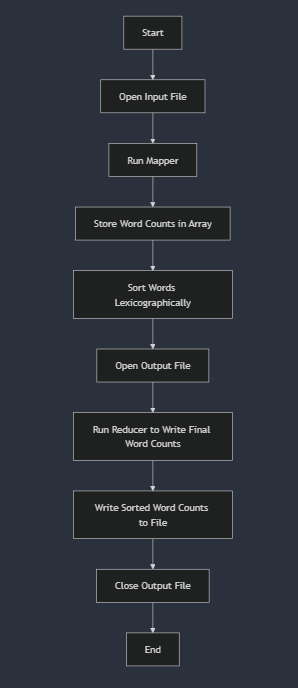
\includegraphics[width=0.8\textwidth]{wordcount-flowchart.png} % Replace with actual diagram file
    \captionof{figure}{Mapper and Reducer Workflow}
\end{center}

\section*{Conclusion}
This implementation showcases a straightforward yet effective use of the MapReduce paradigm for word count. The separation of concerns between the Mapper and Reducer functions highlights the modularity of the approach, making it easy to adapt for larger datasets or distributed systems.

\end{document}
